\documentclass[11pt]{article}

% Packages
\usepackage[margin=1in]{geometry}
\usepackage{amsmath,amssymb}
\usepackage{natbib}
\usepackage{graphicx}
\usepackage{booktabs}
\usepackage{xcolor}
\usepackage{hyperref}
\usepackage{cleveref}
\usepackage{tikz}
\usetikzlibrary{arrows.meta, positioning, calc, fit, backgrounds, shapes.geometric, decorations.pathreplacing}

% Custom commands
\newcommand{\sigextra}{\sigma_{\text{extra}}}
\newcommand{\daT}{\mathrm{d}\alpha/\mathrm{d}T}
\newcommand{\GMSL}{\text{GMSL}}
\newcommand{\GMST}{\text{GMST}}
\newcommand{\CDW}{\text{CDW}}
\newcommand{\ENSO}{\text{ENSO}}

\title{A Hierarchical Bayesian Framework for\\
  Self-Consistent Sea Level Rise Forecasting:\\
  From Global Constraints to Local Projections}

\author{Framework Document — Working Draft}
\date{\today}

\begin{document}
\maketitle

\begin{abstract}
No single approach to sea level rise (SLR) projection is sufficient.  Process models lack systematic parameter exploration and diverge from observations; purely statistical models cannot resolve component-specific dynamics; expert assessments lack formal self-consistency.  We outline a hierarchical Bayesian framework that fuses observational constraints, statistical models, and process-model structural information into a single, self-consistent probabilistic forecast.  The framework operates across four levels: (0)~global temperature forcing, (1)~total GMSL constrained by the observational record, (2)~component-level decomposition with component-specific data and models, and (3)~deep-uncertainty modules for ice-sheet processes.  At each level, posteriors from one analysis become informed priors for the next, and a global budget constraint ensures that components sum to the observed total.  The framework is designed to be built incrementally: it is self-consistent at every stage of completeness, with unresolved components absorbed into a residual term.
\end{abstract}


% ====================================================================
\section{Motivation}
% ====================================================================

Current approaches to SLR projection fall into three broad categories, each with fundamental limitations:

\begin{enumerate}
  \item \textbf{Process models} (e.g., ISMIP6, GlacierMIP): Simulate ice-sheet and glacier dynamics from first principles, but lack systematic parameter exploration, use heuristic parameterisations for key processes (calving, sub-shelf melting), and produce ensembles that immediately diverge from observations after initialisation \citep{fricker2025antarctica}.  Under 4\textdegree C of warming, IPCC AR6 process-model projections show less SLR by 2100 than a simple extrapolation of observed satellite-era trends --- a physically implausible result that reflects structural model deficiencies rather than true uncertainty.

  \item \textbf{Semi-empirical / statistical models} (e.g., Vermeer \& Rahmstorf 2009, this work): Calibrate a rate--temperature relationship against observations, providing strong constraints on the historical period but limited ability to resolve component-specific dynamics or capture nonlinear threshold behaviour (e.g., marine ice-sheet instability).

  \item \textbf{Expert elicitation and structured assessments} (e.g., IPCC AR6, Bamber et al.\ 2019): Synthesise multiple lines of evidence but lack formal probabilistic self-consistency between components and total.
\end{enumerate}

The framework described here aims to combine the strengths of all three approaches while providing formal self-consistency through Bayesian hierarchical modelling.  The central principle is:

\begin{quote}
\emph{Observations constrain the total; component models and data inform the decomposition; the budget ensures consistency; deep-uncertainty modules handle what observations alone cannot resolve.}
\end{quote}


% ====================================================================
\section{Framework Architecture}
% ====================================================================

The framework operates across four levels, connected by Bayesian conditioning and a budget constraint (\cref{fig:dag}).

\begin{figure}[p]
\centering
\resizebox{\textwidth}{!}{%
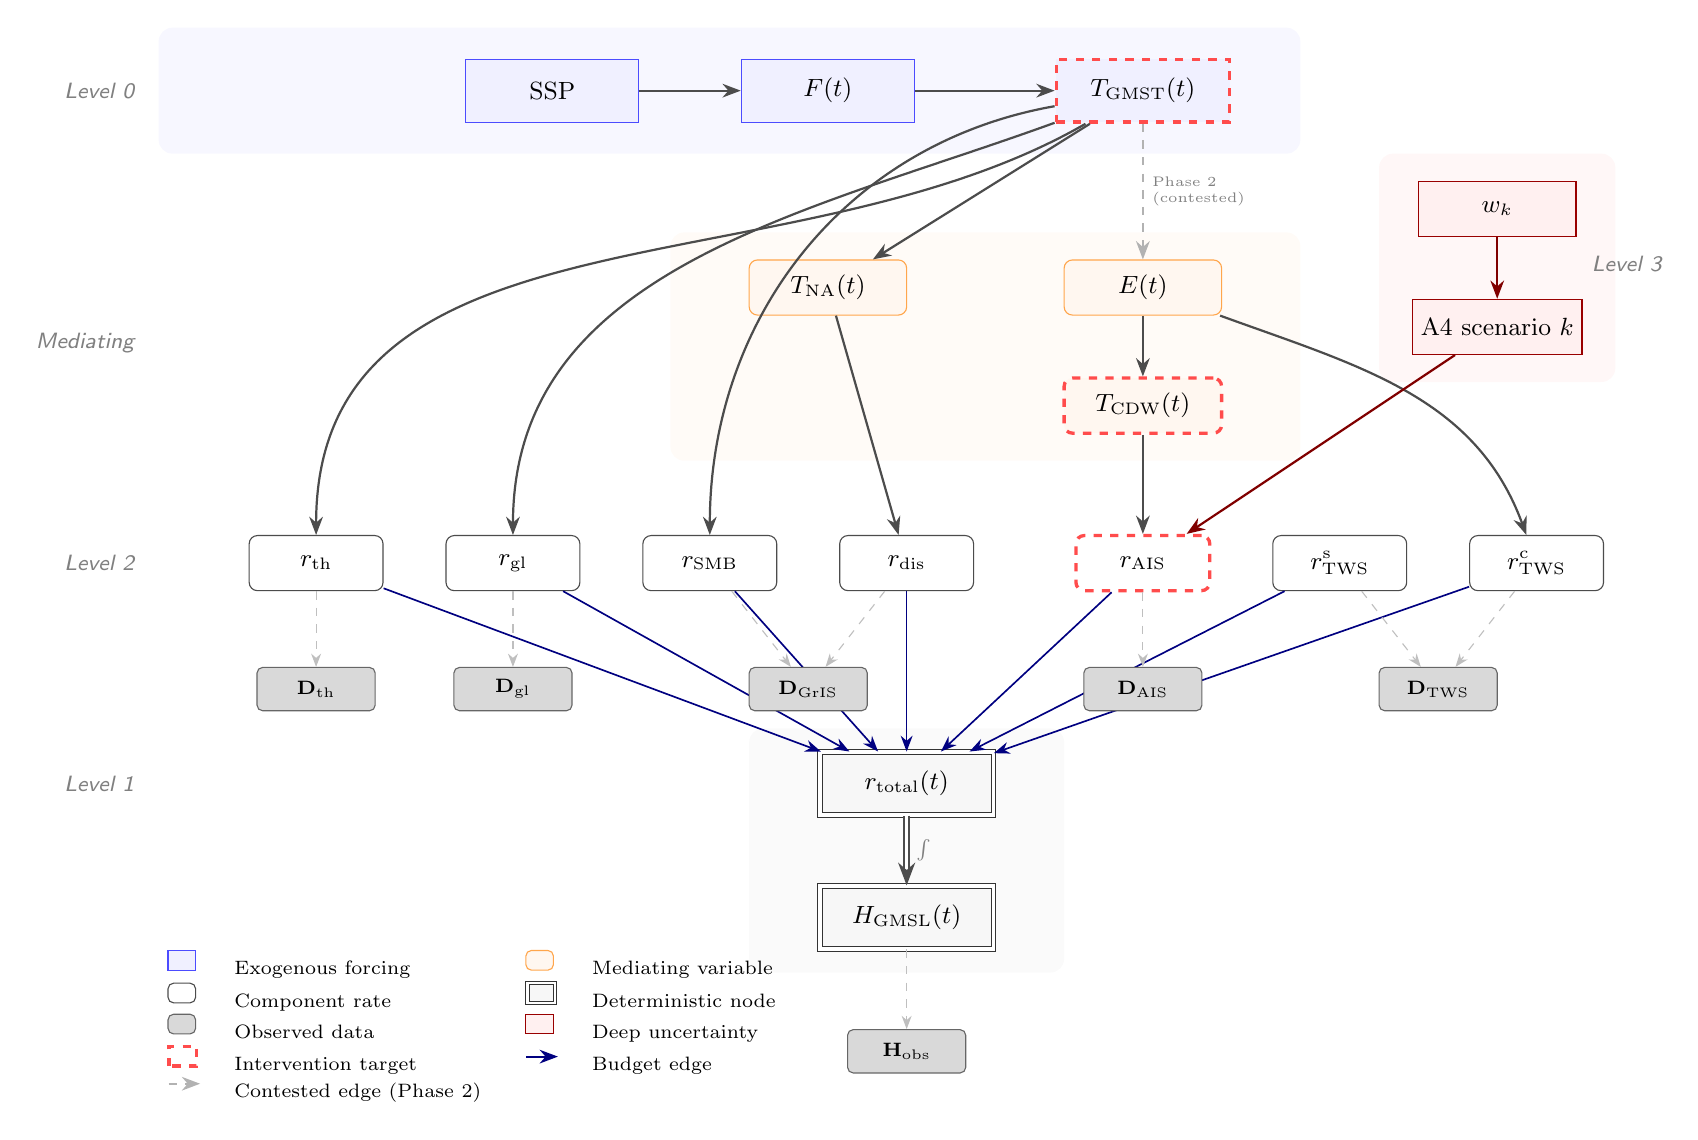
\begin{tikzpicture}[
  % Base settings
  >=Stealth,
  every node/.append style={inner sep=3pt},
  % --- Node styles ---
  forcing/.style={rectangle, draw=blue!70, fill=blue!6,
    minimum width=2.2cm, minimum height=0.8cm, font=\small, align=center},
  mediating/.style={rectangle, rounded corners=3pt, draw=orange!70, fill=orange!6,
    minimum width=2cm, minimum height=0.7cm, font=\small, align=center},
  component/.style={rectangle, rounded corners=3pt, draw=black!70, fill=white,
    minimum width=1.7cm, minimum height=0.7cm, font=\small, align=center},
  determ/.style={rectangle, draw=black!80, fill=gray!6, double, double distance=1.2pt,
    minimum width=2.2cm, minimum height=0.8cm, font=\small, align=center},
  observed/.style={rectangle, rounded corners=2pt, draw=black!60, fill=gray!30,
    minimum width=1.5cm, minimum height=0.55cm, font=\scriptsize, align=center},
  deep/.style={rectangle, draw=red!60!black, fill=red!6,
    minimum width=2cm, minimum height=0.7cm, font=\small, align=center},
  % --- Edge styles ---
  causal/.style={->, thick, black!70},
  budget_edge/.style={->, semithick, blue!50!black},
  obs_edge/.style={->, thin, gray!50, dashed},
  deep_edge/.style={->, thick, red!50!black},
  % --- Intervention marker ---
  interv/.style={draw=red!70, very thick, dashed},
  % --- Labels ---
  levellab/.style={font=\footnotesize\sffamily\itshape, text=black!50, anchor=east},
]

% ============================================================
% LEVEL 0: External forcing (top row)
% ============================================================
\node[forcing] (ssp) at (-4, 10) {SSP};
\node[forcing] (F)   at (-0.5, 10) {$F(t)$};
\node[forcing, interv] (T) at (3.5, 10) {$T_{\GMST}(t)$};

\draw[causal] (ssp) -- (F);
\draw[causal] (F) -- (T);

% ============================================================
% MEDIATING VARIABLES
% ============================================================
\node[mediating] (Tna) at (-0.5, 7.5) {$T_{\text{NA}}(t)$};
\node[mediating] (enso) at (3.5, 7.5) {$E(t)$};
\node[mediating, interv] (Tcdw) at (3.5, 6) {$T_{\CDW}(t)$};

% Level 0 --> Mediating
\draw[causal] (T) -- (Tna);
\draw[causal, dashed, gray!60] (T) -- (enso)
  node[midway, right, font=\tiny, text=black!50, align=left] {Phase 2\\(contested)};
\draw[causal] (enso) -- (Tcdw);

% ============================================================
% LEVEL 3: Deep uncertainty (right column)
% ============================================================
\node[deep] (wk) at (8, 8.5) {$w_k$};
\node[deep] (a4) at (8, 7) {A4 scenario $k$};

\draw[deep_edge] (wk) -- (a4);

% ============================================================
% LEVEL 2: Component rates (main row)
% ============================================================
% GMST-forced (left group)
\node[component] (rth)  at (-7, 4) {$r_{\text{th}}$};
\node[component] (rgl)  at (-4.5, 4) {$r_{\text{gl}}$};
\node[component] (rsmb) at (-2, 4) {$r_{\text{SMB}}$};
% Ocean-forced (centre)
\node[component] (rdis) at (0.5, 4) {$r_{\text{dis}}$};
\node[component, interv] (rais) at (3.5, 4) {$r_{\text{AIS}}$};
% TWS (right group)
\node[component] (rtws_s) at (6, 4) {$r_{\text{TWS}}^{\text{s}}$};
\node[component] (rtws_c) at (8.5, 4) {$r_{\text{TWS}}^{\text{c}}$};

% Level 0 --> Level 2 (direct GMST forcing)
\draw[causal] (T) to[out=-150, in=90] (rth);
\draw[causal] (T) to[out=-160, in=90] (rgl);
\draw[causal] (T) to[out=-170, in=90] (rsmb);

% Mediating --> Level 2
\draw[causal] (Tna) -- (rdis);
\draw[causal] (Tcdw) -- (rais);
\draw[causal] (enso) to[out=-20, in=110] (rtws_c);

% Level 3 --> Level 2
\draw[deep_edge] (a4) -- (rais);

% ============================================================
% LEVEL 1: Budget constraint and GMSL (bottom centre)
% ============================================================
\node[determ] (rtot) at (0.5, 1.2) {$r_{\text{total}}(t)$};
\node[determ] (H) at (0.5, -0.5) {$H_{\GMSL}(t)$};

\draw[causal, double, double distance=1pt] (rtot) -- (H)
  node[midway, right, font=\scriptsize, text=black!50] {$\int$};

% Level 2 --> Level 1 (budget sum)
\draw[budget_edge] (rth)  -- (rtot);
\draw[budget_edge] (rgl)  -- (rtot);
\draw[budget_edge] (rsmb) -- (rtot);
\draw[budget_edge] (rdis) -- (rtot);
\draw[budget_edge] (rais) -- (rtot);
\draw[budget_edge] (rtws_s) -- (rtot);
\draw[budget_edge] (rtws_c) -- (rtot);

% ============================================================
% OBSERVATION NODES (shaded)
% ============================================================
\node[observed] (Hobs)  at (0.5, -2.2) {$\mathbf{H}_{\text{obs}}$};
\node[observed] (Dth)   at (-7, 2.4) {$\mathbf{D}_{\text{th}}$};
\node[observed] (Dgl)   at (-4.5, 2.4) {$\mathbf{D}_{\text{gl}}$};
\node[observed] (Dgris) at (-0.75, 2.4) {$\mathbf{D}_{\text{GrIS}}$};
\node[observed] (Dais)  at (3.5, 2.4) {$\mathbf{D}_{\text{AIS}}$};
\node[observed] (Dtws)  at (7.25, 2.4) {$\mathbf{D}_{\text{TWS}}$};

% Observation edges (generative direction: latent --> observed)
\draw[obs_edge] (H) -- (Hobs);
\draw[obs_edge] (rth) -- (Dth);
\draw[obs_edge] (rgl) -- (Dgl);
\draw[obs_edge] (rsmb) -- (Dgris);
\draw[obs_edge] (rdis) -- (Dgris);
\draw[obs_edge] (rais) -- (Dais);
\draw[obs_edge] (rtws_s) -- (Dtws);
\draw[obs_edge] (rtws_c) -- (Dtws);

% ============================================================
% LEVEL LABELS (left margin)
% ============================================================
\node[levellab] at (-9.2, 10) {Level 0};
\node[levellab] at (-9.2, 6.8) {Mediating};
\node[levellab] at (-9.2, 4) {Level 2};
\node[levellab] at (-9.2, 1.2) {Level 1};
\node[levellab] at (10.2, 7.8) {Level 3};

% ============================================================
% BACKGROUND SHADING (level bands)
% ============================================================
\begin{scope}[on background layer]
  \fill[blue!3, rounded corners=5pt] (-9, 9.2) rectangle (5.5, 10.8);
  \fill[orange!3, rounded corners=5pt] (-2.5, 5.3) rectangle (5.5, 8.2);
  \fill[white, rounded corners=5pt] (-8.5, 3.2) rectangle (10, 4.8);
  \fill[gray!4, rounded corners=5pt] (-1.5, -1.2) rectangle (2.5, 1.9);
  \fill[red!3, rounded corners=5pt] (6.5, 6.3) rectangle (9.5, 9.2);
\end{scope}

% ============================================================
% LEGEND
% ============================================================
\node[anchor=north west, font=\scriptsize] at (-9, -0.8) {%
  \begin{tabular}{@{}ll@{\qquad}ll@{}}
    \tikz[baseline=-0.5ex]\draw[fill=blue!6, draw=blue!70] (0,0) rectangle (0.35,0.25); & Exogenous forcing &
    \tikz[baseline=-0.5ex]\draw[fill=orange!6, draw=orange!70, rounded corners=2pt] (0,0) rectangle (0.35,0.25); & Mediating variable \\
    \tikz[baseline=-0.5ex]\draw[fill=white, draw=black!70, rounded corners=2pt] (0,0) rectangle (0.35,0.25); & Component rate &
    \tikz[baseline=-0.5ex]\draw[fill=gray!6, draw=black!80, double, double distance=0.8pt] (0,0) rectangle (0.35,0.25); & Deterministic node \\
    \tikz[baseline=-0.5ex]\draw[fill=gray!30, draw=black!60, rounded corners=2pt] (0,0) rectangle (0.35,0.25); & Observed data &
    \tikz[baseline=-0.5ex]\draw[fill=red!6, draw=red!60!black] (0,0) rectangle (0.35,0.25); & Deep uncertainty \\
    \tikz[baseline=-0.5ex]\draw[red!70, very thick, dashed] (0,0) rectangle (0.35,0.25); & Intervention target &
    \tikz[baseline=-0.5ex]\draw[->, thick, blue!50!black] (0,0.12) -- (0.4,0.12); & Budget edge \\
    \tikz[baseline=-0.5ex]\draw[->, thick, dashed, gray!60] (0,0.12) -- (0.4,0.12); & Contested edge (Phase 2) & &  \\
  \end{tabular}};

\end{tikzpicture}
}% end resizebox
\caption{Directed acyclic graph of the hierarchical framework.  Nodes are grouped by level: Level~0 (exogenous forcing, blue), Level~2 (component rates, white), Level~1 (budget constraint and GMSL, gray, double-bordered), and Level~3 (deep uncertainty, red).  Orange nodes are mediating variables that transmit forcing from Level~0 to specific Level~2 components via physically distinct pathways.  Shaded gray nodes are observed data.  Dashed red borders mark intervention targets for causal counterfactuals (\cref{tab:interventions}).  Blue edges denote the rate-level budget constraint (soft likelihood, \cref{eq:budget-constraint}).  Dashed gray edges are generative observation models.  The dashed edge $T_{\GMST} \to E(t)$ is contested and inactive in Phase~1: ENSO is treated as exogenous (see text).  Notation: $r_{\text{th}}$~= thermosteric rate; $r_{\text{gl}}$~= glacier rate; $r_{\text{SMB}}$, $r_{\text{dis}}$~= GrIS surface mass balance and discharge rates; $r_{\text{AIS}}$~= AIS rate; $r_{\text{TWS}}^{\text{s}}$, $r_{\text{TWS}}^{\text{c}}$~= TWS secular and climate-driven rates; $E(t)$~= ENSO index; $T_{\text{NA}}$~= North Atlantic SST proxy; $T_{\CDW}$~= Circumpolar Deep Water temperature proxy.}
\label{fig:dag}
\end{figure}

\subsection{Level 0: External forcing}

Temperature forcing $T(t)$ is treated as an external input, drawn from CMIP6 / IPCC assessed ranges for each SSP scenario.  The across-scenario spread contributes $\sigma_{\text{scenario}}^2$ to the total projection uncertainty.  Temperature is not a free parameter of the SLR model; it is conditioned upon.

\subsection{Level 1: Global GMSL constraint}

The polynomial rate--temperature model
\begin{equation}
  \text{rate}(t) = a\,T(t)^2 + b\,T(t) + c, \qquad
  H(t) = H_0 + \int_0^t \text{rate}(\tau)\,\mathrm{d}\tau
  \label{eq:rate-model}
\end{equation}
is calibrated against the full $\sim$119-year GMSL record using a Bayesian level-space approach (companion document).  An Exponential (PC) prior on~$a$ provides genuine shrinkage toward the order-1 model, letting the data determine whether quadratic acceleration is supported.  A rate-and-state extension with relaxation time~$\tau$ captures lagged response from slow ocean and ice-sheet processes.

The Level~1 posterior provides:
\begin{itemize}
  \item A calibrated total rate at any temperature, with uncertainty;
  \item A total GMSL projection envelope $\sigma_{\text{constrained}}^2$;
  \item A \emph{budget}: the sum of all component rates must equal the Level~1 total within posterior uncertainty.
\end{itemize}

\subsection{Level 2: Component decomposition}

The total rate is decomposed into contributions from distinct physical processes:
\begin{equation}
  \text{rate}_{\text{total}}(t) = \text{rate}_{\text{thermo}}(t)
    + \text{rate}_{\text{glaciers}}(t)
    + \text{rate}_{\text{GrIS}}(t)
    + \text{rate}_{\text{AIS}}(t)
    + \text{rate}_{\text{TWS}}(t)
  \label{eq:budget}
\end{equation}
Each component defines its own rate model with its own physically appropriate forcing variable(s) (\cref{tab:component-models}).  The components are not required to share a common polynomial-in-$T$ parameterisation; the only structural requirement is that their rates sum to the observed total.

The budget constraint enters the joint model as a \emph{soft likelihood} rather than a deterministic parameter identity.  At each observation time $t_j$ in the calibration period:
\begin{equation}
  \text{rate}_{\text{total}}(t_j) - \sum_{i=1}^{K} \text{rate}_i(t_j)
  \sim \mathcal{N}\!\left(0,\; \sigma_{\text{budget}}^2(t_j)\right)
  \label{eq:budget-constraint}
\end{equation}
where
\begin{equation}
  \sigma_{\text{budget}}^2(t_j) = \sigma_{\text{obs,total}}^2(t_j) + \sum_{i=1}^{K} \sigma_{\text{extra},i}^2
  \label{eq:budget-tolerance}
\end{equation}
incorporates both the measurement uncertainty in the total GMSL rate and the component-level model inadequacy terms $\sigma_{\text{extra},i}$ (\cref{sec:component-discrepancy}).  In the limit $\sigma_{\text{budget}} \to 0$, this recovers the deterministic budget; allowing slight imbalance prevents numerical pathologies from degenerate posteriors while honestly reflecting that no finite set of component models perfectly accounts for every physical process contributing to the total.

This soft-constraint formulation follows the approach to constraints in Bayesian calibration problems described by \citet{kennedy2001bayesian} and \citet{brynjarsdottir2014learning}.  The budget acts as both a \emph{regulariser} (preventing components from drifting to implausible values) and a \emph{cross-component constraint} (well-observed components tighten the residual and thereby constrain poorly observed ones).  Critically, because the constraint operates at every time step rather than through a small number of shared polynomial parameters, the regularisation is stronger: it penalises component models that deviate from the total \emph{anywhere} in the calibration period, not only through their integrated polynomial behaviour.

\subsection{Level 3: Deep-uncertainty modules}

For components where observational constraints are insufficient to characterise the tails of the distribution --- principally the Antarctic Ice Sheet --- structured deep-uncertainty modules extend the projection envelope.  The A4 scenario-mixture framework (companion document) provides a physically motivated, discrete mixture of ice-sheet futures:
\begin{itemize}
  \item S1: Status quo (no marine ice-sheet instability);
  \item S2: Marine ice-sheet instability (MISI);
  \item S3: MISI with amplifying feedbacks;
  \item S4: MISI with marine ice-cliff instability (MICI).
\end{itemize}
Each scenario has its own within-scenario distribution; the mixture weights encode expert assessment of scenario plausibility.  The resulting deep-uncertainty contribution enters the total projection variance through the nested law-of-total-variance decomposition (\cref{sec:variance}).  The approximation that the A4 contribution is independent of the Level~1 calibration uncertainty (Assumption~V1 in~\cref{sec:variance-approx}) requires that the A4 scenarios be consistent with the historical budget residual; this condition is tested empirically.

\subsection{Formal DAG specification}
\label{sec:dag-spec}

The DAG in \cref{fig:dag} encodes the causal assumptions of the framework.  This subsection specifies all nodes, edges, implied conditional independence relations, and intervention targets.  The specification serves three purposes: (1)~it makes the conditional independence structure of the joint posterior (\cref{eq:joint-posterior}) explicit and verifiable; (2)~it defines which nodes support do-operations for counterfactual analysis; and (3)~it provides the formal object against which any future extension of the framework must be checked for consistency.

\subsubsection{Node set}

\begin{table}[ht]
\centering
\caption{Complete node set of the framework DAG.  Node types: \textbf{F}~= exogenous forcing (Level~0), \textbf{M}~= mediating variable, \textbf{C}~= component rate (Level~2), \textbf{G}~= global constraint (Level~1), \textbf{D}~= deep uncertainty (Level~3), \textbf{O}~= observed data.}
\label{tab:dag-nodes}
\small
\begin{tabular}{lllp{7cm}}
\toprule
Node & Symbol & Type & Description \\
\midrule
SSP scenario & SSP & F & Shared Socioeconomic Pathway label; indexes the forcing trajectory.  Discrete. \\
Radiative forcing & $F(t)$ & F & Net anthropogenic radiative forcing (W\,m$^{-2}$), conditioned on SSP. \\
Global mean temperature & $T_{\GMST}(t)$ & F & Global mean surface temperature anomaly relative to pre-industrial. \\
\addlinespace
North Atlantic SST proxy & $T_{\text{NA}}(t)$ & M & Subsurface ocean temperature relevant to GrIS marine-terminating outlet glaciers.  Mediates GMST $\to$ GrIS discharge. \\
ENSO index & $E(t)$ & M & El Ni\~no--Southern Oscillation state (e.g., Ni\~no~3.4 index or SOI).  Mediates multiple cross-component couplings. \\
CDW temperature proxy & $T_{\CDW}(t)$ & M & Circumpolar Deep Water temperature on the Antarctic continental shelf.  Mediates ENSO $\to$ AIS forcing. \\
\addlinespace
Thermosteric rate & $r_{\text{th}}(t)$ & C & Ocean thermal expansion rate (mm\,yr$^{-1}$). \\
Glacier rate & $r_{\text{gl}}(t)$ & C & Glaciers and ice caps mass-loss rate (mm\,yr$^{-1}$ SLE). \\
GrIS SMB rate & $r_{\text{SMB}}(t)$ & C & Greenland surface mass balance rate. \\
GrIS discharge rate & $r_{\text{dis}}(t)$ & C & Greenland ice discharge rate (marine-terminating outlet glaciers). \\
AIS rate & $r_{\text{AIS}}(t)$ & C & Antarctic Ice Sheet mass-loss rate.  Budget residual during calibration; A4 module during projection. \\
TWS secular rate & $r_{\text{TWS}}^{\text{s}}(t)$ & C & Terrestrial water storage secular rate (dams, groundwater). \\
TWS climate rate & $r_{\text{TWS}}^{\text{c}}(t)$ & C & Terrestrial water storage climate-driven rate (ENSO-mediated). \\
\addlinespace
Total rate & $r_{\text{total}}(t)$ & G & Deterministic sum of component rates (\cref{eq:budget}).  Constrained via soft likelihood (\cref{eq:budget-constraint}). \\
GMSL & $H_{\GMSL}(t)$ & G & Global mean sea level, obtained by integrating $r_{\text{total}}$. \\
\addlinespace
A4 scenario index & $k$ & D & Discrete index over AIS deep-uncertainty scenarios (S1--S4). \\
Scenario weights & $w_k$ & D & Prior mixture weights from expert assessment; updated by budget consistency. \\
\addlinespace
GMSL observations & $\mathbf{H}_{\text{obs}}$ & O & Frederikse et al.\ (2020) reconstruction, 1900--2018. \\
Component datasets & $\mathbf{D}_{\text{th}}, \mathbf{D}_{\text{gl}}, \mathbf{D}_{\text{GrIS}}, \mathbf{D}_{\text{AIS}}, \mathbf{D}_{\text{TWS}}$ & O & Component-specific observational records (Argo, GlaMBIE, IMBIE, GRACE, etc.). \\
\bottomrule
\end{tabular}
\end{table}

\subsubsection{Edge set}

The directed edges encode generative (causal) relationships.  Each edge $A \to B$ asserts that $B$ is generated by a mechanism that takes $A$ as input; the conditional distribution $p(B \mid \mathrm{pa}(B))$ is part of the joint model specification.

\paragraph{Forcing chain (Level~0).}
$\text{SSP} \to F(t) \to T_{\GMST}(t)$.  Radiative forcing is determined by the SSP scenario; GMST responds to forcing via the climate system (treated as a known input, not a free parameter of the SLR model).

\paragraph{GMST $\to$ component rates (direct).}
$T_{\GMST} \to r_{\text{th}}$, $T_{\GMST} \to r_{\text{gl}}$, $T_{\GMST} \to r_{\text{SMB}}$.  These components respond directly to global mean temperature through thermodynamic mechanisms (thermal expansion, surface energy balance, melt).

\paragraph{GMST $\to$ mediating variables.}
$T_{\GMST} \to T_{\text{NA}}$: GMST influences North Atlantic subsurface temperature, mediated by Atlantic Meridional Overturning Circulation and regional ocean dynamics.  $T_{\GMST} \to E(t)$: warming may shift ENSO statistics \citep{cai2014increasing}, but the hypothesis is not robustly supported by CMIP6 multi-model ensembles, which show no agreement on the sign or magnitude of the ENSO response to warming.  \textbf{Phase~1 treatment}: ENSO is exogenous.  The $T_{\GMST} \to E(t)$ edge is \emph{inactive}: ENSO statistics are drawn from the historical record or from a specified scenario, not generated endogenously by the model.  This means that do-interventions on $F(t)$ (SAI, CDR) do \emph{not} propagate to $r_{\text{AIS}}$ or $r_{\text{TWS}}^{\text{c}}$ via ENSO in Phase~1.  The edge will be activated in Phase~2 with a mandatory sensitivity analysis comparing counterfactual projections with and without the edge active (see~\cref{fig:dag}, where the edge is shown dashed).

\paragraph{Teleconnection edges.}
$T_{\text{NA}} \to r_{\text{dis}}$: ocean thermal forcing on marine-terminating Greenland outlet glaciers \citep{straneo2013north}.  $E(t) \to T_{\CDW}$: ENSO modulates CDW delivery to the Antarctic continental shelf via the Pacific--South American teleconnection \citep{steig2012tropical, paolo2018response}.  $T_{\CDW} \to r_{\text{AIS}}$: sub-shelf basal melt rates respond to CDW temperature.  $E(t) \to r_{\text{TWS}}^{\text{c}}$: ENSO drives terrestrial water storage variability through precipitation shifts.

\paragraph{Budget edges (deterministic).}
$\{r_{\text{th}}, r_{\text{gl}}, r_{\text{SMB}}, r_{\text{dis}}, r_{\text{AIS}}, r_{\text{TWS}}^{\text{s}}, r_{\text{TWS}}^{\text{c}}\} \to r_{\text{total}}$: the total rate is the deterministic sum of component rates.  $r_{\text{total}} \to H_{\GMSL}$: GMSL is the time integral of the total rate.

\paragraph{Deep-uncertainty edges (Level~3).}
$w_k \to k$: the A4 scenario index is drawn from the categorical distribution defined by the mixture weights.  $k \to r_{\text{AIS}}$: the A4 scenario determines the AIS rate distribution during projection.  \emph{Future edge (Phase~2)}: the Glen--Nye flow law exponent $n$ (sampled from a prior on $[3, 4]$) will modify the within-scenario AIS rate distributions via a rheology correction following the analysis of \citet{getraer2025glen}.  The edge $n \to r_{\text{AIS}}$ couples the A4 projection to ice rheology uncertainty, which is currently treated as an implicit structural assumption within each A4 scenario rather than as a sampled parameter.

\paragraph{Observation edges (generative).}
$H_{\GMSL} \to \mathbf{H}_{\text{obs}}$: the GMSL observation model (measurement noise + datum uncertainty).  $r_i \to \mathbf{D}_i$ for each component with direct observations: the component-specific measurement models.  Note that $\mathbf{D}_{\text{GrIS}}$ is generated jointly by $r_{\text{SMB}}$ and $r_{\text{dis}}$, and $\mathbf{D}_{\text{TWS}}$ is generated jointly by $r_{\text{TWS}}^{\text{s}}$ and $r_{\text{TWS}}^{\text{c}}$.

\subsubsection{Conditional independence structure}
\label{sec:ci}

The DAG implies the following conditional independence (CI) relations.  Each is stated with its physical justification and the conditions under which it could be violated.

\paragraph{Critical distinction: generative vs.\ inferential dependence.}
The CI relations below describe the \emph{generative} model --- the data-generating process assumed by the framework.  During \emph{inference}, the dependence structure is different, and the difference is central to how the framework operates.  The total rate node $r_{\text{total}}$ is a \emph{collider}: all seven component rates feed into it via the budget sum.  In the generative model, where $r_{\text{total}}$ is unobserved, the component rates are d-separated from each other given their respective forcings (see CI-1--CI-3 below).  However, during inference, $r_{\text{total}}$ is effectively conditioned upon, because the GMSL likelihood $p(\mathbf{H}_{\text{obs}} \mid \ldots)$ constrains $H_{\GMSL}(t) = \int r_{\text{total}}(\tau)\,\mathrm{d}\tau$.  By the rules of d-separation, conditioning on a collider \emph{opens} paths between its parents that were previously blocked.  Concretely: once the total rate is constrained by the GMSL observations, learning that one component rate is large forces the remaining components to be collectively smaller, and vice versa.

This collider-induced coupling is not a pathology --- it is the \emph{mechanism} by which the budget constraint creates cross-component information flow.  It is the formal graphical-model statement of the ``top-down constraint'' described in~\cref{sec:mechanics}: well-constrained components (e.g., thermosteric) tighten the budget residual and thereby indirectly constrain poorly observed components (e.g., AIS).  The CI relations below hold in the generative model but are systematically violated during inference.  Where this violation is substantive, it is noted explicitly.

\begin{enumerate}
  \item \textbf{CI-1}: $r_{\text{th}} \perp\!\!\!\perp r_{\text{AIS}} \mid T_{\GMST}, E(t)$.  The thermosteric rate is independent of the AIS rate given GMST and ENSO state.  \emph{Justification}: the only coupling is through shared forcing; there is no direct thermosteric $\to$ AIS or AIS $\to$ thermosteric mechanism.  \emph{Potential violation}: freshwater input from AIS mass loss could modify ocean stratification and thereby affect thermosteric expansion at regional scales.  This is a second-order effect that is negligible at the global level over the calibration period but could become relevant under high-end AIS loss scenarios.  \emph{Inferential violation}: conditioning on $r_{\text{total}}$ (via $\mathbf{H}_{\text{obs}}$) opens the collider path $r_{\text{th}} \to r_{\text{total}} \leftarrow r_{\text{AIS}}$.  During inference, the thermosteric and AIS rates become negatively correlated: a posterior draw in which the thermosteric rate is higher than expected leaves less budget residual for AIS, and vice versa.  This is precisely the mechanism by which the well-constrained Argo-era thermosteric estimate tightens the AIS contribution.

  \item \textbf{CI-2}: $r_{\text{TWS}}^{\text{c}} \perp\!\!\!\perp r_{\text{AIS}} \mid E(t)$.  The climate-driven TWS rate and the AIS rate are conditionally independent given ENSO state.  \emph{Justification}: ENSO is the sole common driver; no direct TWS $\to$ AIS or AIS $\to$ TWS pathway exists.  \emph{Potential violation}: if additional unmodelled climate modes (e.g., Indian Ocean Dipole, SAM) simultaneously affect both TWS and CDW delivery, the CI relation is approximate.  This is mitigated by the fact that ENSO is the dominant mode on the relevant timescales.  \emph{Inferential violation}: same collider mechanism as CI-1.  Conditioning on the budget total induces posterior correlation between $r_{\text{TWS}}^{\text{c}}$ and $r_{\text{AIS}}$ even when ENSO is conditioned upon.  The induced correlation is weaker than for CI-1 because $r_{\text{TWS}}^{\text{c}}$ has smaller magnitude, but it is structurally present in the posterior.

  \item \textbf{CI-3}: $r_{\text{gl}} \perp\!\!\!\perp r_{\text{dis}} \mid T_{\GMST}$.  Glacier rate is independent of GrIS discharge rate given GMST.  \emph{Justification}: glacier melt responds to atmospheric temperature; GrIS discharge responds to North Atlantic ocean temperature.  Both are driven by GMST but through different mechanisms with no direct cross-pathway.  \emph{Potential violation}: high-latitude glacier mass loss (e.g., Svalbard, Iceland) may share regional ocean forcing with Greenland marine-terminating glaciers.  This is a regional effect absorbed by the model-inadequacy terms.

  \item \textbf{CI-4}: $\mathbf{D}_i \perp\!\!\!\perp \mathbf{D}_j \mid r_i, r_j$ for $i \neq j$ when the datasets are instrumentally independent.  \emph{Justification}: given the true component rates, the measurement errors are independent if the instruments are distinct.  \emph{Potential violation}: GRACE provides mass-change estimates for glaciers, GrIS, AIS, and TWS simultaneously; if the GRACE processing introduces correlated errors across these products, CI-4 is violated for GRACE-derived datasets.  This must be handled by a correlated error model for GRACE components (deferred to Phase~2 unless cross-product GRACE correlations are large enough to affect the posterior).

  \item \textbf{CI-5}: $r_{\text{TWS}}^{\text{s}} \perp\!\!\!\perp r_i \mid$ nothing, for all $i \neq \text{TWS}^{\text{s}}$.  The secular TWS rate has no parents in the DAG other than its own parameters; it is marginally independent of all climate-driven rates.  \emph{Justification}: dam impoundment and groundwater extraction are driven by human decisions, not by climate forcing.  This is the strongest CI assumption in the framework and is well-supported physically.
\end{enumerate}

\noindent These CI relations should be tested empirically during implementation.  CI-1 and CI-2 can be checked by examining residual correlations between components after conditioning on the relevant forcing variables.  CI-4 requires assessment of GRACE inter-product error correlations.  The collider-induced inferential violations of CI-1 through CI-3 and CI-5 are not testable in the usual sense --- they are structural consequences of conditioning on the budget constraint and are present by construction.  They can, however, be \emph{quantified} by computing pairwise posterior correlations $\text{Cor}[r_i(t), r_j(t) \mid \mathbf{H}_{\text{obs}}, \mathbf{D}]$ and comparing to the generative prior correlations.  The difference measures the strength of the top-down budget regularisation at each time step.  Large inferential correlations indicate times where the budget is doing substantial work to constrain the decomposition; small correlations indicate times where the component-specific data are sufficient on their own.

\subsubsection{Intervention targets}
\label{sec:interventions}

For causal counterfactual analysis --- specifically, for evaluating proposed glacier stabilisation interventions under the Ar\^ete Glacier Initiative --- certain nodes must be manipulable via Pearl's do-operator \citep{pearl2009causality}.  A do-operation $do(X = x)$ replaces the natural generative mechanism for $X$ (i.e., deletes all incoming edges to $X$) and fixes $X$ at the specified value.  The post-intervention distribution is obtained by graph surgery on the DAG.

\begin{table}[ht]
\centering
\caption{Intervention targets and their DAG operations.  Each intervention corresponds to a do-operation on a specific node, with the specified incoming edges severed.}
\label{tab:interventions}
\small
\begin{tabular}{p{3.2cm}p{4.5cm}p{5.5cm}}
\toprule
Intervention & DAG operation & Downstream effects \\
\midrule
Stabilise Thwaites grounding line & $do(r_{\text{AIS}} = f_{\text{stab}}(t))$ where $f_{\text{stab}}$ specifies the stabilised trajectory.  Severs $T_{\CDW} \to r_{\text{AIS}}$ and $k \to r_{\text{AIS}}$. & $r_{\text{total}}$, $H_{\GMSL}$ change; all other component rates unaffected. \\
\addlinespace
Reduce basal melt via MCB & $do(T_{\CDW} = T_{\CDW} - \Delta T_{\text{MCB}})$.  Severs $E(t) \to T_{\CDW}$; replaces with modified mechanism. & $r_{\text{AIS}}$ responds through the $T_{\CDW} \to r_{\text{AIS}}$ edge; cascades to $r_{\text{total}}$, $H_{\GMSL}$.  Other components unaffected unless MCB also modifies $E(t)$. \\
\addlinespace
Stratospheric aerosol injection & $do(F(t) = F_{\text{SAI}}(t))$.  Severs SSP $\to F(t)$; replaces with modified forcing trajectory. & $T_{\GMST}$ changes; GMST-forced components ($r_{\text{th}}$, $r_{\text{gl}}$, $r_{\text{SMB}}$) and $r_{\text{dis}}$ (via $T_{\text{NA}}$) respond directly.  \textbf{Phase~1}: with ENSO exogenous, SAI does \emph{not} propagate to $r_{\text{AIS}}$ or $r_{\text{TWS}}^{\text{c}}$ via the ENSO pathway.  \textbf{Phase~2}: with $T_{\GMST} \to E(t)$ active, SAI additionally propagates through ENSO to $r_{\text{TWS}}^{\text{c}}$ and to $r_{\text{AIS}}$ via $E(t) \to T_{\CDW}$. \\
\addlinespace
Carbon dioxide removal & $do(F(t) = F_{\text{CDR}}(t))$.  Same structural operation as SAI but different temporal profile. & Same propagation as SAI (including the Phase~1/Phase~2 distinction regarding the ENSO pathway); slower onset, persistent effect. \\
\addlinespace
Combined CDR + MCB & $do(F(t) = F_{\text{CDR}}(t)),\; do(T_{\CDW} = g(T_{\CDW}, \text{MCB}))$.  Simultaneous intervention on two nodes. & Global forcing reduction (via CDR) plus targeted Antarctic shelf cooling (via MCB).  The DAG structure permits computing the joint effect because the two intervention targets have no common descendant that is also an ancestor of the other. \\
\bottomrule
\end{tabular}
\end{table}

The DAG structure ensures that counterfactual queries are well-defined: for any intervention on any marked node, the post-intervention distribution is uniquely determined by the truncated factorisation \citep{pearl2009causality}.  The key requirement is that the causal mechanisms encoded by the edges are \emph{autonomous} --- that is, intervening on one mechanism does not alter others.  This autonomy assumption is defensible for the interventions in \cref{tab:interventions}: stabilising a grounding line does not alter the physics of thermal expansion, and modifying radiative forcing does not alter the dam-impoundment history.

\paragraph{Phase 1 limitation.}  In Phase~1, the component rate models are statistical (polynomial, linear, or index-based), not mechanistic.  This means that counterfactual queries that push the forcing far outside the calibration range will produce extrapolations whose reliability depends on the structural correctness of the statistical model.  Phase~2 (emulator-based component models) will address this by replacing statistical rate models with emulators trained on mechanistic simulators, which have more defensible extrapolation behaviour within their domain of physical validity.

\paragraph{Value-of-information queryability.}  The DAG structure determines which observations reduce uncertainty on which projections.  For any hypothetical future observation at node~$X$, the set of downstream nodes whose posterior variance would be reduced can be identified by graph-theoretic computation on the DAG without re-running inference: it is the set of nodes reachable from~$X$ in the moral graph induced by the current evidence set.  This property supports value-of-information (VoI) analysis for observational investment decisions (Phase~3).  The Phase~1 design decisions that preserve this capability are: (i)~forward models accept arbitrary $(t)$ evaluation points, not only the observation grid; (ii)~the likelihood interface supports appending hypothetical observations by specifying type, time, value, and uncertainty; (iii)~MCMC outputs store full parameter vectors and per-observation log-likelihoods to enable importance reweighting under hypothetical data augmentation.


% ====================================================================
\section{Component Models and Informed Priors}
\label{sec:components}
% ====================================================================

\begin{table}[ht]
\centering
\caption{Component rate models and forcing variables.  Each component defines its own functional form with its own physically appropriate forcing; no shared polynomial-in-$T$ parameterisation is imposed.}
\label{tab:component-models}
\begin{tabular}{llll}
\toprule
Component & Rate model & Forcing variable(s) & Justification \\
\midrule
Thermosteric & $b_{\text{th}} T + c_{\text{th}}$ & GMST & Direct thermodynamic response \\
Glaciers & $(a_{\text{gl}} T^2 + b_{\text{gl}} T + c_{\text{gl}})\cdot[V_{\text{gl}}/V_{\text{gl},0}]^p$ & GMST & Melt + area-loss + depletion \\
GrIS (SMB) & $b_{\text{SMB}} T + c_{\text{SMB}}$ & GMST & Surface energy balance \\
GrIS (discharge) & $\beta_{\text{dis}} T_{\text{NA}} + c_{\text{dis}}$ & North Atlantic SST & Ocean-forced outlet dynamics \\
AIS & Budget residual (calibration); & CDW proxy & Ocean-forced dynamics \\
    & A4 module (projection) & & \\
TWS (secular) & $c_{\text{TWS}}$ & Dam/GW records & No temperature dependence \\
TWS (climate) & $\gamma_{\text{TWS}} \cdot E(t)$ & ENSO index & Precipitation-mediated \\
\bottomrule
\end{tabular}
\end{table}

Each component analysis provides a marginal posterior on its own parameters, which serves as an \emph{informed prior} when incorporated into the joint hierarchical model.  The strength of the prior reflects the quality and length of the component-specific observational record.  Because the budget operates at the rate level (\cref{eq:budget-constraint}), components are not required to share a parameterisation; each uses the functional form and forcing variables most appropriate to its physics (\cref{tab:component-models}).

\subsection{Thermosteric expansion}
\label{sec:thermo}

\paragraph{Data.}  Argo float array (2005--present, global coverage below 2000~m); ocean reanalysis products (1950--present, declining coverage with depth and time); XBT profiles (1960s--present, upper 700~m, with known fall-rate biases).

\paragraph{Model.}  Thermal expansion is well-understood from first principles: $\text{rate}_{\text{thermo}}(T) \approx b_{\text{th}} \cdot T + c_{\text{th}}$.  The response is expected to be nearly linear in global mean temperature because the thermal expansion coefficient varies slowly over the relevant temperature range.  A quadratic term $a_{\text{th}} T^2$ is available but expected to be small; an Exponential (PC) prior on $a_{\text{th}}$ provides shrinkage toward the linear model.  A scalar model-inadequacy term $\sigma_{\text{extra,th}}$ (\cref{sec:scalar-discrepancy}) accounts for unmodeled variability, primarily from depth-dependent heat uptake dynamics and regional ocean circulation effects.

\paragraph{Phase~2 model extension: deep-ocean lag.}  The linear-in-$T$ model captures the upper-ocean response but ignores the slow equilibration of the deep ocean.  If Phase~1 residuals show structure consistent with a lagged response, a two-timescale model should replace the linear model: $\text{rate}_{\text{th}}(t) = b_{\text{fast}} T(t) + b_{\text{slow}} S_{\text{deep}}(t)$, with $\mathrm{d}S_{\text{deep}}/\mathrm{d}t = (T(t) - S_{\text{deep}}(t))/\tau_{\text{deep}}$ and $\tau_{\text{deep}} \sim 200$--1000~yr.  This is a \emph{model extension} (not a discrepancy correction) that captures the committed thermosteric response from heat already in the system.  It is deferred to Phase~2 unless the Phase~1 thermosteric residual diagnostics indicate structured model error.

\paragraph{Prior contribution.}  Because thermal expansion is the best-constrained component, the prior on $b_{\text{th}}$ will be tight: approximately Normal($\mu_{\text{th}}, \sigma_{\text{th}}$) with $\sigma_{\text{th}}$ determined by the Argo-era uncertainty.  This tight prior propagates through the rate-level budget to constrain the residual available to other components at every calibration time step.

\subsection{Glaciers and ice caps}
\label{sec:glaciers}

\paragraph{Data.}  Randolph Glacier Inventory (RGI); geodetic mass balance estimates; GRACE/GRACE-FO (2002--present); regional temperature and precipitation records.

\paragraph{Model.}  Glacier mass balance responds to both temperature (melt) and precipitation (accumulation).  The temperature sensitivity may be nonlinear because: (a)~small glaciers disappear entirely, reducing the total glacier area; (b)~the elevation--temperature feedback amplifies warming at glacier surfaces.  A polynomial rate model $\text{rate}_{\text{glaciers}}^{\text{uncorrected}}(T) = a_{\text{gl}} \cdot T^2 + b_{\text{gl}} \cdot T + c_{\text{gl}}$, with $a_{\text{gl}} > 0$ reflecting the accelerating loss as glacier area shrinks, captures the historical temperature sensitivity but is unphysical for projection: the global glacier reservoir is finite ($\sim$0.32~m sea level equivalent), and the polynomial model extrapolates monotonically increasing loss rates even after the reservoir is substantially depleted.

\paragraph{Volume-depletion saturation.}  The forward model must include a volume-depletion correction that bounds the cumulative glacier contribution by the remaining glacier volume:
\begin{equation}
  \text{rate}_{\text{glaciers}}(t) = \left(a_{\text{gl}} T^2 + b_{\text{gl}} T + c_{\text{gl}}\right)
    \cdot \left[\frac{V_{\text{gl}}(t)}{V_{\text{gl},0}}\right]^{p}
  \label{eq:glacier-depletion}
\end{equation}
where $V_{\text{gl},0} \approx 0.32$~m SLE is the initial (reference-epoch) total glacier volume, $V_{\text{gl}}(t) = V_{\text{gl},0} - \int_0^t \text{rate}_{\text{glaciers}}(\tau)\,\mathrm{d}\tau$ is the remaining volume at time~$t$, and the exponent $p > 0$ controls how sharply the rate declines as the reservoir depletes.

This is a \emph{forward model extension}, not a discrepancy correction: without it, the model produces physically impossible projections above $\sim$3\textdegree C of warming (cumulative loss exceeding the total reservoir).  The depletion factor is unity at the start of the calibration period and declines monotonically; it has negligible effect during the historical period (when $V_{\text{gl}}(t) \approx V_{\text{gl},0}$) but dominates the projection at high warming levels.

The exponent $p$ is calibrated, with a prior informed by the glacier volume--area scaling relationships used in GlacierMIP \citep{marzeion2012past, edwards2021projected}: $p \sim \text{LogNormal}(\log 0.7, 0.3)$, reflecting expectation that the rate declines somewhat more slowly than linearly with remaining volume (because large glaciers persist longer than small ones, and the area-weighted sensitivity shifts as small glaciers disappear).

\paragraph{Prior contribution.}  Moderate constraint on $b_{\text{gl}}$ from the geodetic record; weak constraint on $a_{\text{gl}}$ from the relatively short satellite era.  The key question is whether the observed glacier acceleration is separable from ice-sheet acceleration in the GRACE record.  The depletion exponent $p$ is weakly constrained by the historical record (negligible depletion to date) and must be informed by the prior from glacier model intercomparisons.

\subsection{Greenland Ice Sheet}
\label{sec:gris}

\paragraph{Data.}  GRACE/GRACE-FO; SMB models (RACMO, MAR); ice discharge estimates from satellite velocity and thickness.

\paragraph{Model.}  Greenland mass loss has two distinct channels: surface mass balance (SMB, strongly temperature-dependent) and ice discharge (driven primarily by ocean--ice interaction at marine-terminating outlet glaciers).  A two-component model:
\begin{equation}
  \text{rate}_{\text{GrIS}}(t) = \underbrace{b_{\text{SMB}} \cdot T(t) + c_{\text{SMB}}}_{\text{SMB (GMST-forced)}} + \underbrace{\beta_{\text{dis}} \cdot T_{\text{NA}}(t) + c_{\text{dis}}}_{\text{Discharge (ocean-forced)}}
\end{equation}
where $T_{\text{NA}}(t)$ is a North Atlantic ocean temperature proxy.  The discharge term is driven by ocean thermal forcing on marine-terminating outlet glaciers, not by GMST directly; the relationship between GMST and North Atlantic subsurface temperature is mediated by Atlantic meridional overturning and regional ocean dynamics.  During the pre-Argo era, $T_{\text{NA}}$ may need to be treated as a latent variable or parameterised as a function of GMST with substantial uncertainty.

\paragraph{Prior contribution.}  The SMB component provides an informed prior on $b_{\text{SMB}}$ from regional climate models (RACMO, MAR); the discharge component contributes through $\beta_{\text{dis}}$ and $c_{\text{dis}}$, constrained by satellite-era velocity and thickness observations.  Separate model-inadequacy terms $\sigma_{\text{extra,SMB}}$ and $\sigma_{\text{extra,dis}}$ (\cref{sec:scalar-discrepancy}) account for unmodeled variability in each channel: for SMB, primarily precipitation effects and melt--albedo feedbacks not captured by the linear model; for discharge, poorly characterised pre-Argo ocean forcing and nonlinear calving dynamics.

\subsection{Antarctic Ice Sheet}
\label{sec:ais}

\paragraph{Data.}  GRACE/GRACE-FO; altimetry (CryoSat-2, ICESat-2); InSAR-derived ice velocities; ocean temperature observations on the continental shelf.

\paragraph{Model.}  The AIS contribution is the least constrained and most consequential for high-end projections.  The historical contribution ($\sim$0.3~mm/yr, $\sim$8--9\% of the total GMSL rate) is small relative to the observational uncertainty, and the future trajectory depends on poorly constrained processes (marine ice-sheet instability, ice-cliff failure, sub-shelf melting parameterisation).

In the hierarchical framework, the AIS operates at two levels:
\begin{itemize}
  \item \textbf{Budget-constrained estimate}: The Level~1 total minus the sum of better-constrained components yields a \emph{residual} that bounds the historical AIS contribution.  This is an indirect but powerful constraint.
  \item \textbf{Deep-uncertainty extension}: The A4 scenario-mixture module (Level~3) extends the projection envelope beyond what the historical record can constrain.
\end{itemize}

\paragraph{Prior contribution.}  The AIS rate is \emph{not} modelled as a polynomial in GMST.  Dynamical mass loss is driven by ocean thermal forcing on the Antarctic continental shelf --- warm Circumpolar Deep Water (\CDW) intrusions modulated by atmospheric teleconnections (Pacific--South American pattern, Southern Annular Mode) and ocean circulation --- and the relationship between GMST and \CDW{} temperature at the Amundsen Sea grounding zones is neither linear nor monotonic.  During calibration, the AIS contribution is primarily constrained by the budget residual: the Level~1 total minus the sum of all better-constrained components.  During projection, the A4 module (Level~3) provides the AIS rate distribution conditioned on scenario.  The budget residual provides indirect but powerful constraint: any systematic bias in the AIS rate would manifest as a misfit to the total GMSL record propagated through the budget likelihood (\cref{eq:budget-constraint}).

\subsection{Terrestrial water storage}
\label{sec:tws}

\paragraph{Data.}  GRACE/GRACE-FO; dam construction records; groundwater depletion estimates; land hydrology models.

\paragraph{Model.}  TWS is often treated as a purely non-climatic contribution (dam impoundment, groundwater extraction), contributing only to the background rate~$c$.  This is an oversimplification.  TWS has both secular and climate-driven components:
\begin{equation}
  \text{rate}_{\text{TWS}}(t) = c_{\text{TWS,secular}} + \text{rate}_{\text{TWS,climate}}(t)
  \label{eq:tws}
\end{equation}

\paragraph{Climate-driven TWS and the ENSO--WAIS teleconnection.}

The climate-driven component of TWS is substantial and coupled to modes of climate variability, particularly the El Ni\~no--Southern Oscillation (ENSO).  ENSO drives large interannual fluctuations in terrestrial water storage through shifts in precipitation patterns, river discharge, and soil moisture.  These fluctuations are visible in both the GRACE TWS record and in GMSL residuals after removing the secular trend.

Critically, ENSO also modulates the delivery of warm Circumpolar Deep Water (\CDW) to the Antarctic continental shelf \citep{steig2012tropical, paolo2018response}.  During El Ni\~no events, anomalous atmospheric circulation patterns (transmitted via the Pacific--South American teleconnection) weaken the westerlies along the Amundsen Sea coast, altering the thermocline depth and allowing warm \CDW{} to reach the grounding zones of Thwaites and Pine Island glaciers.  This drives enhanced basal melting, grounding-line retreat, and --- if sustained --- potentially irreversible marine ice-sheet instability.

The implication for the hierarchical framework is that TWS and AIS are \emph{not independent components}.  The same climate mode (ENSO) that drives short-timescale TWS variability also modulates the ocean forcing that controls WAIS stability on longer timescales.  This coupling operates across timescales:

\begin{itemize}
  \item \textbf{Interannual ($\sim$2--7 yr):} ENSO-driven TWS fluctuations and ENSO-driven \CDW{} intrusions are essentially simultaneous, driven by the same atmospheric teleconnection.  On these timescales, the TWS and AIS signals may partially cancel in the GMSL budget (land water storage increases during La Ni\~na, when \CDW{} intrusions are weaker).

  \item \textbf{Decadal ($\sim$10--30 yr):} Sustained periods of El Ni\~no--like conditions (e.g., the positive phase of the Interdecadal Pacific Oscillation) can drive cumulative grounding-line retreat that crosses irreversibility thresholds.  The TWS signal integrates to near zero over these timescales, but the ice-sheet response is path-dependent and potentially irreversible.

  \item \textbf{Centennial ($\sim$100+ yr):} If anthropogenic warming shifts the mean state of the tropical Pacific toward more frequent or intense El Ni\~no conditions \citep{cai2014increasing}, the time-mean \CDW{} delivery to the Amundsen Sea increases, loading the dice for MISI even in the absence of extreme individual events.
\end{itemize}

\paragraph{Implications for the framework.}

The ENSO--TWS--WAIS coupling has three consequences for the hierarchical model:

\begin{enumerate}
  \item \textbf{Cross-component covariance:} The component decomposition (\cref{eq:budget}) must allow for non-zero covariance between $\text{rate}_{\text{TWS}}$ and $\text{rate}_{\text{AIS}}$ at interannual timescales.  A diagonal error model (independent components) would underestimate the total uncertainty on short timescales and overestimate it on long timescales.

  \item \textbf{State-dependent AIS forcing:} The rate-and-state model's relaxation time $\tau$ may need to be conditioned on ENSO state or its long-term statistics, rather than treated as a fixed parameter.  A regime-dependent $\tau$ (fast response during El Ni\~no, slow during La Ni\~na) could capture the asymmetric forcing.

  \item \textbf{Irreversibility and path dependence:} The A4 scenario-mixture weights (Level~3) should be informed by the projected evolution of ENSO statistics under warming.  If climate models project more frequent El Ni\~no conditions, the probability weight on S2--S4 (MISI scenarios) should increase, because the cumulative \CDW{} forcing is more likely to trigger irreversible retreat.
\end{enumerate}

\paragraph{Prior contribution.}  TWS contributes an informed prior on $c_{\text{TWS}}$ from dam and groundwater records.  The climate-driven component is parameterised as $\gamma_{\text{TWS}} \cdot E(t)$ where $E(t)$ is an ENSO index, because the TWS--temperature relationship is mediated by ENSO rather than by direct thermodynamic forcing.  Forcing TWS into a polynomial-in-$T$ model would create a spurious temperature dependence that contaminates the budget.


\subsection{Component-level model inadequacy}
\label{sec:component-discrepancy}

The Level~1 model includes a learned model-inadequacy parameter $\sigextra$ that absorbs unmodeled interannual variability (ENSO, volcanic effects, internal climate modes).  The Level~2 component models require an analogous treatment.  Each component rate model (linear-in-$T$ thermosteric, quadratic-in-$T$ glaciers, etc.)\ is a parametric approximation to the true physical rate.  Without a discrepancy term, the parametric model is asserted as exact, forcing the component parameters to absorb variability that should be attributed to model error.  The resulting component posteriors are overconfident, and the budget residual inherits the bias.

\subsubsection{Component discrepancy model}
\label{sec:discrepancy-model}

For each component~$i$, the observed rate is modelled as:
\begin{equation}
  \text{rate}_i^{\text{obs}}(t) = \text{rate}_i^{\text{model}}(t;\, \boldsymbol{\theta}_i) + \delta_i(t) + \epsilon_i(t)
  \label{eq:component-discrepancy}
\end{equation}
where $\text{rate}_i^{\text{model}}(t;\, \boldsymbol{\theta}_i)$ is the parametric forward model (as specified in~\cref{tab:component-models}), $\delta_i(t)$ is the model discrepancy --- the systematic difference between the true rate and the best-fitting parametric model --- and $\epsilon_i(t)$ is the observation noise (measurement error in $\mathbf{D}_i$).

This decomposition follows the framework of \citet{kennedy2001bayesian}: the discrepancy $\delta_i(t)$ is a property of the \emph{model}, not of the observations.  It represents the irreducible gap between the parametric functional form and the true physical rate, evaluated at the true parameter values.  Omitting this term (i.e., setting $\delta_i \equiv 0$) is equivalent to asserting that the parametric model is the true data-generating process, which is not credible for any of the component models.

\subsubsection{Phase~1 implementation: scalar discrepancy}
\label{sec:scalar-discrepancy}

In Phase~1, the discrepancy is represented as a scalar inflation of the component observation variance --- the simplest possible treatment that captures the \emph{magnitude} of model inadequacy without modelling its temporal structure:
\begin{equation}
  \sigma_{D_i,\text{eff}}^2(t_j) = \sigma_{D_i}^2(t_j) + \sigma_{\text{extra},i}^2
  \label{eq:component-variance-inflation}
\end{equation}
where $\sigma_{D_i}^2(t_j)$ is the known measurement uncertainty for component~$i$ at time~$t_j$ (from the component-specific dataset $\mathbf{D}_i$), and $\sigma_{\text{extra},i}$ is a learned parameter representing the root-mean-square amplitude of the model discrepancy for component~$i$.

This is equivalent to treating $\delta_i(t) \sim \mathcal{N}(0, \sigma_{\text{extra},i}^2)$ independently at each time step --- i.e., white-noise discrepancy.  This is conservative in the sense that it inflates the component uncertainty uniformly across time, regardless of whether the model error is concentrated at particular times (e.g., during volcanic eruptions or strong ENSO events).  It cannot capture systematic biases or temporally correlated model errors, which would require the Gaussian process treatment described below.

\paragraph{Priors on $\sigma_{\text{extra},i}$.}  Each $\sigma_{\text{extra},i}$ receives a weakly informative half-Cauchy prior:
\begin{equation}
  \sigma_{\text{extra},i} \sim \text{HalfCauchy}(0,\; s_i)
  \label{eq:discrepancy-prior}
\end{equation}
where the scale~$s_i$ is set to the expected magnitude of unmodeled variability for that component.  Recommended values for Phase~1 (in mm/yr):

\begin{center}
\begin{tabular}{lrl}
\toprule
Component & $s_i$ (mm/yr) & Rationale \\
\midrule
Thermosteric & 0.3 & Best-constrained; residuals expected small \\
Glaciers & 0.5 & Regional variability, precipitation effects \\
GrIS (SMB) & 0.3 & RCM-constrained; moderate residuals \\
GrIS (discharge) & 0.5 & Ocean forcing poorly characterised pre-Argo \\
TWS (secular) & 0.2 & Near-constant; small deviations \\
TWS (climate) & 1.0 & ENSO proxy is imperfect; large interannual signal \\
\bottomrule
\end{tabular}
\end{center}

\noindent These scales are intentionally generous (the half-Cauchy places substantial mass well above the scale parameter) and are designed to let the data determine the posterior.  The AIS component does not receive a separate $\sigma_{\text{extra},i}$ in Phase~1 because the AIS rate is derived as a budget residual during calibration, not fitted to component-specific observations; its model inadequacy is absorbed into the budget tolerance (\cref{eq:budget-tolerance}).

\paragraph{Interaction with the budget tolerance.}  The budget tolerance $\sigma_{\text{budget}}(t_j)$ already includes the $\sigma_{\text{extra},i}$ terms (\cref{eq:budget-tolerance}).  Because the $\sigma_{\text{extra},i}$ are sampled during MCMC, $\sigma_{\text{budget}}$ changes at each iteration.  The sampler must recompute $\sigma_{\text{budget}}$ from the current $\sigma_{\text{extra},i}$ values at each step; it is \emph{not} a pre-computed constant.

\subsubsection{Consistency diagnostic}
\label{sec:discrepancy-consistency}

The sum of component model inadequacies should be approximately consistent with the global model inadequacy:
\begin{equation}
  \sigextra^2 \approx \sum_{i=1}^{K} \sigma_{\text{extra},i}^2
  \label{eq:discrepancy-consistency}
\end{equation}
This is approximate because the global model may have additional (or fewer) sources of inadequacy than the sum of component models --- the global polynomial-in-$T$ model smooths over component-specific variability that the individual models are designed to capture.

\paragraph{Diagnostic (mandatory).}  After the Phase~1 posterior is obtained, compare $\hat{\sigextra}^2$ (the posterior median of the global model inadequacy) with $\sum_i \hat{\sigma}_{\text{extra},i}^2$ (the posterior median of the summed component inadequacies).  Three outcomes are possible:
\begin{enumerate}
  \item $\sum_i \hat{\sigma}_{\text{extra},i}^2 \approx \hat{\sigextra}^2$: The component models collectively account for the same level of model error as the global model.  This is the expected outcome if the component functional forms are well-chosen.
  \item $\sum_i \hat{\sigma}_{\text{extra},i}^2 \gg \hat{\sigextra}^2$: The component models are individually underfit (or the global polynomial captures structure that the components miss through cancellation of correlated errors across components).  Investigate whether cross-component discrepancy correlations provide partial cancellation.
  \item $\sum_i \hat{\sigma}_{\text{extra},i}^2 \ll \hat{\sigextra}^2$: The global model has unmodeled variability that the component decomposition resolves (e.g., because component-specific forcing variables capture variance that the global polynomial-in-$T$ cannot).  This would be evidence that the component decomposition improves the physical representation.
\end{enumerate}

\subsubsection{Phase~2 extension: Gaussian process discrepancy}
\label{sec:gp-discrepancy}

If Phase~1 diagnostics reveal temporally structured residuals in any component's fit (e.g., systematic positive residuals during volcanic recovery periods, or autocorrelated residuals at interannual timescales), the scalar discrepancy should be replaced with a Gaussian process:
\begin{equation}
  \delta_i(t) \sim \mathcal{GP}\!\left(0,\; k_i(t, t';\, \lambda_i, \sigma_{\delta,i})\right)
  \label{eq:gp-discrepancy}
\end{equation}
where $k_i$ is a stationary covariance kernel (Mat\'ern-$\tfrac{5}{2}$ recommended for smooth but flexible discrepancy) with lengthscale $\lambda_i$ and amplitude $\sigma_{\delta,i}$.  This captures both the magnitude and the temporal correlation structure of model error.

The GP discrepancy adds 2--3 hyperparameters per component and requires either GP regression at each MCMC step (computationally expensive for long calibration records) or a basis-function approximation \citep{salter2019uncertainty}.  It is deferred to Phase~2 unless the Phase~1 residual diagnostics provide clear evidence of structured model error in a specific component.

\paragraph{Decision criterion for GP upgrade.}  Compute the Durbin--Watson statistic (or the lag-1 autocorrelation) of the standardised residuals $\hat{\delta}_i(t_j) = (\text{rate}_i^{\text{obs}}(t_j) - \text{rate}_i^{\text{model}}(t_j;\, \hat{\boldsymbol{\theta}}_i)) / \sigma_{D_i,\text{eff}}(t_j)$ for each component.  If the lag-1 autocorrelation exceeds $|\hat{\rho}_1| > 0.3$, the white-noise assumption is violated and the GP discrepancy should be considered for that component.


% ====================================================================
\section{Bayesian Mechanics of the Hierarchy}
\label{sec:mechanics}
% ====================================================================

\subsection{Joint model}

The full hierarchical model has the following structure.  Let $\boldsymbol{\theta}_i$ denote the parameter vector for component~$i$ (with component-specific dimension and interpretation; see~\cref{tab:component-models}), let $\boldsymbol{\theta}_{\text{global}} = (a, b, c, \tau, H_0, \sigextra)$ denote the Level~1 global parameters, and let $\boldsymbol{\sigma}_{\text{extra}} = (\sigma_{\text{extra},1}, \ldots, \sigma_{\text{extra},K})$ denote the component-level model-inadequacy parameters (\cref{sec:component-discrepancy}).  The joint posterior is:
\begin{align}
  &p(\boldsymbol{\theta}_{\text{global}}, \boldsymbol{\theta}_1, \ldots, \boldsymbol{\theta}_K, \boldsymbol{\sigma}_{\text{extra}}, \boldsymbol{\eta} \mid \mathbf{H}_{\text{obs}}, \mathbf{D}_1, \ldots, \mathbf{D}_K) \nonumber \\
  &\quad \propto
  \underbrace{p(\mathbf{H}_{\text{obs}} \mid \boldsymbol{\theta}_{\text{global}}, \boldsymbol{\eta})}_{\text{GMSL likelihood}}
  \cdot \underbrace{\prod_{j=1}^{N_t} p_{\text{budget}}\!\left(\text{rate}_{\text{total}}(t_j) - \sum_{i=1}^{K} \text{rate}_i(t_j;\, \boldsymbol{\theta}_i) \;\middle|\; \sigma_{\text{budget}}(t_j;\, \boldsymbol{\sigma}_{\text{extra}})\right)}_{\text{rate-level budget constraint}} \nonumber \\
  &\qquad \cdot \prod_{i=1}^{K} \underbrace{p(\mathbf{D}_i \mid \boldsymbol{\theta}_i,\, \sigma_{\text{extra},i})}_{\text{component likelihoods}}
  \cdot \prod_{i=1}^{K} \underbrace{p(\boldsymbol{\theta}_i)}_{\text{component priors}}
  \cdot \prod_{i=1}^{K} \underbrace{p(\sigma_{\text{extra},i})}_{\text{discrepancy priors}}
  \cdot \underbrace{p(\boldsymbol{\eta})}_{\text{nuisance priors}}
  \label{eq:joint-posterior}
\end{align}
where $p_{\text{budget}}$ is the Gaussian soft constraint from~\cref{eq:budget-constraint}, $\boldsymbol{\eta}$ collects nuisance parameters, and $\mathbf{D}_i$ is the component-specific dataset.  The budget tolerance $\sigma_{\text{budget}}(t_j;\, \boldsymbol{\sigma}_{\text{extra}})$ is given by~\cref{eq:budget-tolerance} and depends on the current values of the $\sigma_{\text{extra},i}$ at each MCMC step.  Each component likelihood $p(\mathbf{D}_i \mid \boldsymbol{\theta}_i, \sigma_{\text{extra},i})$ uses the inflated observation variance $\sigma_{D_i,\text{eff}}^2(t_j)$ from~\cref{eq:component-variance-inflation}; the discrepancy priors $p(\sigma_{\text{extra},i})$ are half-Cauchy distributions (\cref{eq:discrepancy-prior}).

Two structural differences from a coefficient-level budget formulation deserve emphasis:
\begin{enumerate}
  \item The budget is a \emph{likelihood term}, not a deterministic parameter constraint.  The component parameters $\boldsymbol{\theta}_i$ are not algebraically linked to the global parameters $\boldsymbol{\theta}_{\text{global}}$; they are coupled through the rate-level budget likelihood, which penalises configurations where the component rates fail to sum to the total at any calibration time step.
  \item The component parameter vectors $\boldsymbol{\theta}_i$ have different dimensions and physical interpretations.  There is no requirement that each component parameterises its rate as a polynomial in GMST.  The AIS rate may be a budget residual or a function of \CDW{} temperature; the TWS climate rate may depend on the ENSO index; the GrIS discharge rate may depend on North Atlantic SST.  The only requirement is that each $\text{rate}_i(t;\, \boldsymbol{\theta}_i)$ is evaluable at the calibration time points.
\end{enumerate}

\subsection{Information flow}

Information flows in both directions through the hierarchy:

\paragraph{Bottom-up (component data $\to$ global constraint).}  Each component likelihood $p(\mathbf{D}_i \mid \boldsymbol{\theta}_i, \sigma_{\text{extra},i})$ constrains the component rate at times where component-specific observations are available.  Through the rate-level budget (\cref{eq:budget-constraint}), these component-level constraints propagate upward: well-constrained component rates reduce the residual budget available to other components, effectively tightening the total.

\paragraph{Top-down (global likelihood $\to$ component posteriors).}  The GMSL likelihood constrains the total rate $\text{rate}_{\text{total}}(t)$ at every calibration time step.  Components that are poorly observed directly (e.g., AIS before GRACE) receive indirect constraint from the budget: if the sum of well-observed component rates accounts for most of the observed total, the budget likelihood penalises any component configuration whose residual deviates significantly from the remainder.

\paragraph{Cross-component (budget $\to$ pairwise constraints).}  Even without direct observations of a component, the budget and the posteriors on other components provide information.  For example, if thermosteric + glaciers + GrIS + TWS account for $X \pm \sigma_X$ mm/yr at time~$t$, and the total rate is $Y \pm \sigma_Y$ mm/yr, then the AIS rate is constrained to $Y - X \pm \sqrt{\sigma_Y^2 + \sigma_X^2}$ --- an \emph{observationally derived} estimate of the AIS contribution that requires no ice-sheet model.  Because this constraint operates at every time step, it is substantially more informative than a constraint on a few shared polynomial coefficients: the component rates must match the total \emph{everywhere} in the calibration window, not merely on average.

\subsection{Staged implementation}

The framework is designed to be built incrementally.  At any stage, unresolved components are absorbed into a residual:
\begin{equation}
  \text{rate}_{\text{residual}}(t) = \text{rate}_{\text{total}}(t) - \sum_{i \in \text{resolved}} \text{rate}_i(t)
\end{equation}

\begin{enumerate}
  \item \textbf{Stage 0 (current):} Global GMSL constraint only.  All components are in the residual.  The PC prior on~$a$ and the rate-and-state extension provide the forecasting model.

  \item \textbf{Stage 1:} Add thermosteric decomposition.  This is the best-constrained component and provides the strongest budget constraint on the remaining (primarily cryospheric) residual.

  \item \textbf{Stage 2:} Add glaciers and Greenland.  These are moderately well-observed and further tighten the residual, which now primarily reflects AIS + TWS.

  \item \textbf{Stage 3:} Add TWS (secular and climate-driven components) and the ENSO covariate structure.  The residual now isolates the AIS contribution.

  \item \textbf{Stage 4:} Add AIS with the A4 deep-uncertainty module and the ENSO--\CDW{} coupling.  The framework is now complete.
\end{enumerate}

At each stage, the framework is \emph{self-consistent}: the budget holds, the posteriors are valid, and projections can be made.  Adding a new component \emph{refines} the projections but does not invalidate the previous stage.  Every component enters the framework with its own scalar model-inadequacy term $\sigma_{\text{extra},i}$ (\cref{sec:component-discrepancy}); the discrepancy parameters are sampled jointly with the component parameters from Stage~1 onward.


% ====================================================================
\section{Variance Decomposition and Total Uncertainty}
\label{sec:variance}
% ====================================================================

\subsection{Law of total variance decomposition}

The total GMSL projection $H(t)$ depends on three sources of uncertainty: the SSP scenario index~$S$ (discrete), the A4 deep-uncertainty scenario index~$k$ (discrete), and the Level~1 + Level~2 parameters~$\boldsymbol{\theta}$ (continuous, including both the component model parameters $\boldsymbol{\theta}_i$ and the model-inadequacy parameters $\boldsymbol{\sigma}_{\text{extra}}$; see~\cref{sec:component-discrepancy}).  The total variance is given by iterated application of the law of total variance:
\begin{equation}
  \text{Var}[H(t)]
    = \underbrace{E_S\!\left[\text{Var}_{\boldsymbol{\theta},k}[H(t) \mid S]\right]}_{\text{expected within-scenario variance}}
    + \underbrace{\text{Var}_S\!\left[E_{\boldsymbol{\theta},k}[H(t) \mid S]\right]}_{\text{across-scenario variance}}
  \label{eq:variance-outer}
\end{equation}

The within-scenario variance itself decomposes over the A4 deep-uncertainty structure:
\begin{equation}
  \text{Var}_{\boldsymbol{\theta},k}[H(t) \mid S]
    = \underbrace{E_k\!\left[\text{Var}_{\boldsymbol{\theta}}[H(t) \mid S, k]\right]}_{\text{parameter uncertainty given scenario and A4 regime}}
    + \underbrace{\text{Var}_k\!\left[E_{\boldsymbol{\theta}}[H(t) \mid S, k]\right]}_{\text{across-A4-scenario variance given SSP}}
  \label{eq:variance-inner}
\end{equation}

Here $\text{Var}_{\boldsymbol{\theta}}[H(t) \mid S, k]$ is the posterior parameter uncertainty for a fixed SSP and A4 regime, and $\text{Var}_k[\cdot]$ captures the structural disagreement among A4 scenarios about the AIS contribution.  This nested structure is the correct generalization of the decomposition used by \citet{kopp2014probabilistic}; it replaces the informal additive form that appeared in an earlier draft.

\subsection{Cross-component covariance}

Because $H(t)$ is obtained by integrating the sum of component rates, the parameter-uncertainty term in~\cref{eq:variance-inner} inherits cross-component structure:
\begin{equation}
  \text{Var}_{\boldsymbol{\theta}}\!\left[\sum_i r_i(t) \;\middle|\; S, k\right]
    = \sum_i \text{Var}_{\boldsymbol{\theta}}[r_i(t)]
    + C_{\text{cross}}(t)
  \label{eq:cross-cov}
\end{equation}
where
\begin{equation}
  C_{\text{cross}}(t) = 2 \sum_{i < j} \text{Cov}_{\boldsymbol{\theta}}[r_i(t),\, r_j(t)]
  \label{eq:Ccross}
\end{equation}

The quantity $C_{\text{cross}}(t)$ is a sum of covariances, \emph{not} a variance.  It can be negative (anti-correlated components partially cancel) or positive (correlated amplification).  The notation $\sigma_{\text{cross}}^2$ used in an earlier draft was incorrect because it implied a non-negative quantity.

The dominant contributor to $C_{\text{cross}}$ is $\text{Cov}[r_{\text{TWS,clim}},\, r_{\text{AIS}}]$, which is negative on interannual timescales (La~Ni\~na increases land water storage while reducing CDW intrusions) and may be positive on centennial timescales (sustained El~Ni\~no--like conditions drive both TWS fluctuations and cumulative grounding-line retreat; see~\cref{sec:tws}).

In practice, $C_{\text{cross}}(t)$ is computed directly from the MCMC posterior samples: at each draw~$\boldsymbol{\theta}^{(m)}$, evaluate all component rates and compute the sample covariance across draws.  No analytic approximation is required.  Under the Phase~1 scalar discrepancy model (\cref{sec:scalar-discrepancy}), the component-level model inadequacies are independent by construction (the $\sigma_{\text{extra},i}$ are white-noise terms with no cross-component correlation).  If Phase~2 introduces GP discrepancy (\cref{sec:gp-discrepancy}), cross-component discrepancy correlations become possible (e.g., if a volcanic eruption produces correlated model errors in thermosteric and glacier components), and the total budget-level model inadequacy (\cref{eq:budget-tolerance}) must be augmented with the off-diagonal terms:
\begin{equation}
  \sigma_{\text{budget-inad}}^2(t) = \sum_i \sigma_{\text{extra},i}^2 + 2 \sum_{i < j} \text{Cov}[\delta_i(t),\, \delta_j(t)]
  \label{eq:budget-inad-full}
\end{equation}
Under Phase~1 (independent scalar discrepancy), the covariance terms vanish and~\cref{eq:budget-tolerance} is exact.

\subsection{Conditions for the additive approximation}
\label{sec:variance-approx}

The informal additive form $\sigma_{\text{total}}^2 \approx \sigma_{\text{constrained}}^2 + \sigma_{\text{scenario}}^2 + \sigma_{\text{ice}}^2 + C_{\text{cross}}$ is not wrong as an approximation, but it requires two conditions that must be stated explicitly and checked empirically.

\paragraph{Assumption~V1 (A4/calibration independence).}
$\text{Var}_{\boldsymbol{\theta}}[H(t) \mid S, k]$ and $\text{Var}_k[E_{\boldsymbol{\theta}}[H(t) \mid S, k]]$ are approximately independent --- i.e., the posterior parameter uncertainty does not depend strongly on which A4 scenario is assumed.  This holds if the A4 module does not substantially modify the AIS rate during the calibration period, which in turn requires that the A4 scenarios are consistent with the historical budget residual.  The A4/budget consistency diagnostic (Section~\ref{sec:a4-consistency}\footnote{Section to be added per Item~4 of the revision plan; until then, this forward reference is intentional.}) tests this condition.  If A4 posterior weights differ substantially from prior weights, Assumption~V1 may be violated.

\paragraph{Assumption~V2 (parameter--scenario separability).}
The across-scenario variance $\text{Var}_S[E_{\boldsymbol{\theta},k}[H(t) \mid S]]$ is approximately separable from the parameter uncertainty --- i.e., the temperature-to-rate mapping is approximately the same at the posterior mean as it is over the full posterior.  This holds if the posterior on the rate--temperature relationship is tight enough that nonlinear parameter--temperature interactions are small.

This is a testable condition.  Define the separability ratio:
\begin{equation}
  R_{\text{sep}}(t, S) = \frac{\text{Var}_{\boldsymbol{\theta}}[r(t;\, \boldsymbol{\theta}) \mid S,\, T_S(t)]}
    {\text{Var}_S[r(t;\, \bar{\boldsymbol{\theta}}) \mid \bar{\boldsymbol{\theta}}]}
  \label{eq:Rsep}
\end{equation}
where $\bar{\boldsymbol{\theta}}$ is the posterior mean.  The numerator measures parameter uncertainty at a fixed scenario temperature; the denominator measures scenario spread evaluated at the posterior mean.

% TODO [REVISIT]: The threshold R_sep > 0.3 is a heuristic, not derived from
% first principles.  It encodes the judgment that parameter-temperature
% interaction matters when parameter uncertainty exceeds 30% of scenario spread.
% Once the Phase 1 posterior is available, consider replacing this with a
% data-driven threshold based on the actual posterior predictive distribution,
% e.g., by comparing the full nested variance to the additive approximation
% and setting the threshold where the relative error exceeds some tolerance
% (say 5% or 10% of total Var[H(t)]).  See also: sensitivity of projection
% credible intervals to the choice of decomposition method.
\emph{Diagnostic (mandatory):} Compute $R_{\text{sep}}(t, S)$ at $t \in \{2050, 2100, 2150\}$ for each SSP scenario.  If $R_{\text{sep}} > 0.3$ for any scenario at any horizon, the interaction between parameter uncertainty and scenario spread is non-negligible, and the full nested decomposition (\cref{eq:variance-outer,eq:variance-inner}) must be used rather than the additive approximation.  Report $R_{\text{sep}}$ values in the results.

\subsection{Practical computation}

In practice, the full nested decomposition is computed by Monte Carlo.  For each SSP scenario~$S$:
\begin{enumerate}
  \item Draw $M$ posterior parameter samples $\boldsymbol{\theta}^{(1)}, \ldots, \boldsymbol{\theta}^{(M)}$.
  \item For each draw, sample an A4 scenario~$k$ from its (posterior-updated) categorical distribution.
  \item Evaluate $H^{(m)}(t) = H(t;\, \boldsymbol{\theta}^{(m)}, k^{(m)}, S)$.
  \item The within-scenario variance is $\widehat{\text{Var}}[H(t) \mid S] = \frac{1}{M-1}\sum_m \left(H^{(m)}(t) - \bar{H}_S(t)\right)^2$.
\end{enumerate}
The across-scenario variance is computed from the scenario-specific means $\bar{H}_S(t)$.  The law-of-total-variance decomposition is then exact up to Monte Carlo error, with no approximations required.  The additive approximation and the $R_{\text{sep}}$ diagnostic serve as interpretive tools, not as computational shortcuts.

As the framework matures through the staged implementation, the parameter uncertainty decreases (tighter priors from component decomposition), while the A4 contribution and $C_{\text{cross}}$ become better characterised.


% ====================================================================
\section{Connection to Process Models}
\label{sec:process-models}
% ====================================================================

The framework provides a principled interface to process models that avoids treating their outputs as ground truth:

\begin{enumerate}
  \item \textbf{Structural information $\to$ priors:} Process models (ISMIP6, GlacierMIP) inform the \emph{shape} of component priors: the sign constraints, the expected functional form (linear vs.\ nonlinear), the approximate magnitude.  They do \emph{not} determine the prior location or width, which come from observations.

  \item \textbf{Budget as reality check:} If a process model predicts the AIS rate to be $r_{\text{AIS}} \in [0, 1.5]$~mm/yr over 2005--2020 but the budget-constrained residual implies $r_{\text{AIS}} \in [0.5, 2.5]$~mm/yr, the tension is informative: either the process model is missing physics that accelerates ice loss, or the statistical decomposition is misattributing acceleration from another component.

  \item \textbf{Scenario weights from process understanding:} The A4 mixture weights (Level~3) are informed by process-model ensembles and expert assessment, not by the historical calibration.  This is appropriate because the deep-uncertainty scenarios represent futures that have not yet been observed.

  \item \textbf{Forecast skill evaluation:} The framework provides a natural basis for evaluating process-model forecasting skill.  A process model that predicts component rates inconsistent with the budget-constrained posterior (after accounting for known biases) demonstrates a lack of forecasting skill for that component.
\end{enumerate}


% ====================================================================
\section{Relation to Existing Work}
\label{sec:existing}
% ====================================================================

\paragraph{Semi-empirical models.}  The Vermeer \& Rahmstorf (2009) model $\text{rate} = a \cdot T + b \cdot \mathrm{d}T/\mathrm{d}t$ is a special case of the rate-and-state formulation (companion document shows $b_{\text{VR09}} = -d\tau$ in the small-$\tau$ limit).  The hierarchical framework generalises this by decomposing the global relationship into physically distinct components.

\paragraph{IPCC AR6.}  The AR6 assessed likely ranges are derived from process-model ensembles with expert adjustment.  Our framework can incorporate these ranges as informative priors on component contributions, while using the observational budget as an independent consistency check.  Where the AR6 ranges are inconsistent with the budget, the framework quantifies the tension.

\paragraph{Kopp et al.\ (2014, 2017) and related frameworks.}  The localised probabilistic projections of \citet{kopp2014probabilistic} use a similar component decomposition but without the global budget constraint from a rate--temperature calibration.  Our framework adds this top-level constraint, which provides cross-component regularisation that purely bottom-up approaches lack.


% ====================================================================
\section{Implementation Roadmap}
\label{sec:roadmap}
% ====================================================================

\begin{table}[ht]
\centering
\caption{Staged implementation of the hierarchical framework.}
\label{tab:roadmap}
\begin{tabular}{clll}
\toprule
Stage & Component added & Key data & Status \\
\midrule
0 & Global GMSL--GMST constraint & Frederikse GMSL, Berkeley T & Complete \\
  & \quad + PC prior on $a$, rate-and-state & & Complete \\
  & \quad + A4 deep-uncertainty module & IPCC, expert assessment & Complete \\
1 & Thermosteric decomposition & Argo, ocean reanalysis & Planned \\
2 & Glaciers + Greenland & RGI, GRACE, SMB models & Planned \\
3 & TWS (secular + ENSO-driven) & GRACE, dam/GW records, SOI & Planned \\
4 & AIS + ENSO--\CDW{} coupling & GRACE, altimetry, ocean T & Planned \\
\bottomrule
\end{tabular}
\end{table}


% ====================================================================
\section{Summary}
\label{sec:summary}
% ====================================================================

The hierarchical framework provides:

\begin{enumerate}
  \item \textbf{Self-consistency:} The rate-level budget constraint (\cref{eq:budget,eq:budget-constraint}) ensures that component rates sum to the observed total at every calibration time step, at every stage of implementation.

  \item \textbf{Principled uncertainty:} Bayesian priors encode physical knowledge (sign constraints, PC shrinkage, component-specific data), and the posterior honestly reflects what the observations support.  Learned model-inadequacy terms at both the global (\cref{sec:mechanics}) and component (\cref{sec:component-discrepancy}) levels prevent overconfident posteriors by explicitly acknowledging that no parametric forward model is exact.

  \item \textbf{Incremental refinement:} Each new component tightens the projections without invalidating previous work.  The residual term absorbs unresolved components.

  \item \textbf{Process-model interface:} Process models inform priors and scenario weights but are not treated as ground truth.  The budget provides an independent reality check.

  \item \textbf{Cross-component coupling:} The ENSO--TWS--WAIS teleconnection is explicitly represented, rather than assumed away by a diagonal error model.

  \item \textbf{Transparent prior sensitivity:} The PC prior on~$a$ and the prior predictive checking ensure that the influence of the prior on projections is visible and quantifiable.
\end{enumerate}

The framework is designed not to produce a single ``best estimate'' of future SLR, but to provide a \emph{defensible probabilistic envelope} that honestly reflects what is known, what is uncertain, and what is deeply uncertain --- and to do so in a way that is formally self-consistent across scales, components, and methodological approaches.


\bibliographystyle{apalike}
% \bibliography{references}  % uncomment when .bib is available

\end{document}
